\newpage
\section{Ergebnis}
Nach Abschluss der Realisierung wollen wir in diesem Abschnitt die Ergebnisse vorstellen. Dazu haben wir Screenshots der Oberflächen beider Anwendungen angefertigt, die wir im Folgenden beschreiben. Dabei begründen wir auch Abweichungen, die sich im Vergleich mit den Entwürfen aus dem Anforderungskapitel ergeben haben.

\subsection{Admin}
Die Admin-Oberfläche besteht auch im Ergebnis aus einem Tab-Layout, welches das Umschalten zwischen den drei Reitern ermöglicht und den ausgewählten farblich hervorhebt. Darüber hinaus wurden sämtliche Buttons mit aussagekräftigen Farben versehen, so sind positive Buttons grün, negative Buttons rot und neutrale Buttons blau.

\begin{figure}[H]
\centering
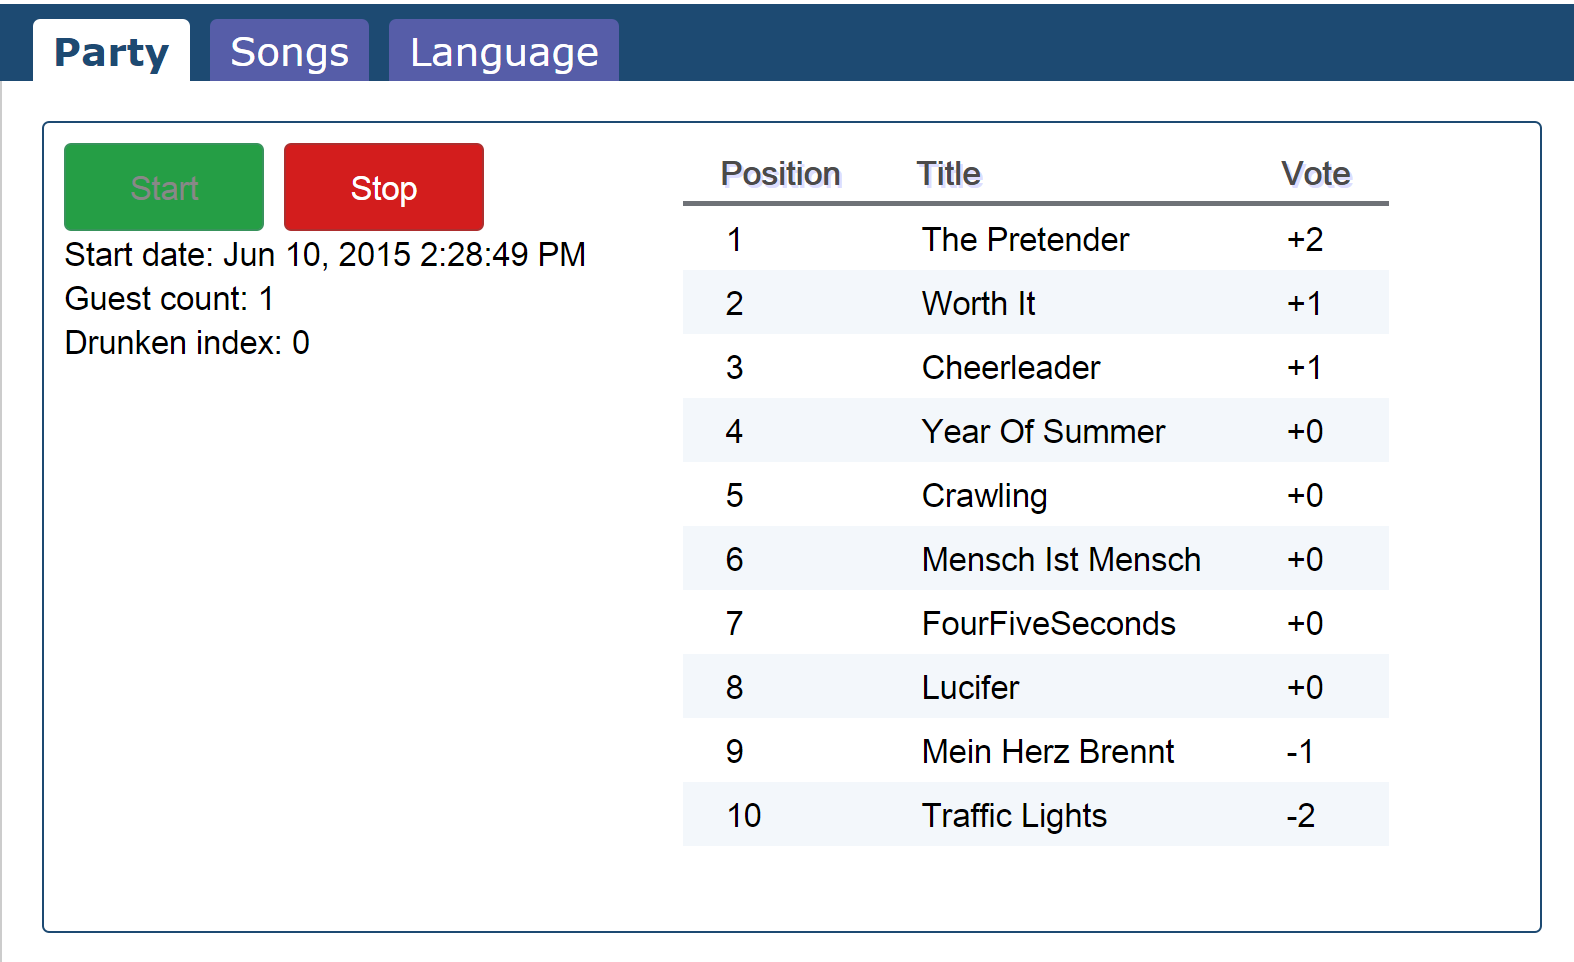
\includegraphics[width=0.9\linewidth]{Bilder/Screenshot-Admin-Party}
\caption{Screenshot der Oberfläche zur Partyverwaltung}
\label{fig:Screenshot-Admin-Party}
\end{figure}

Abbildung \ref{fig:Screenshot-Admin-Party} zeigt die Verwaltungsoberfläche der Party aus der Admin-Applikation. Im Vergleich zum Entwurf (Abb. \ref{fig:MockParty}) liegen die Buttons anstatt unter der Songauflistung nun auf der linken Seite oberhalb der Party-Informationen.

\begin{figure}[H]
\centering
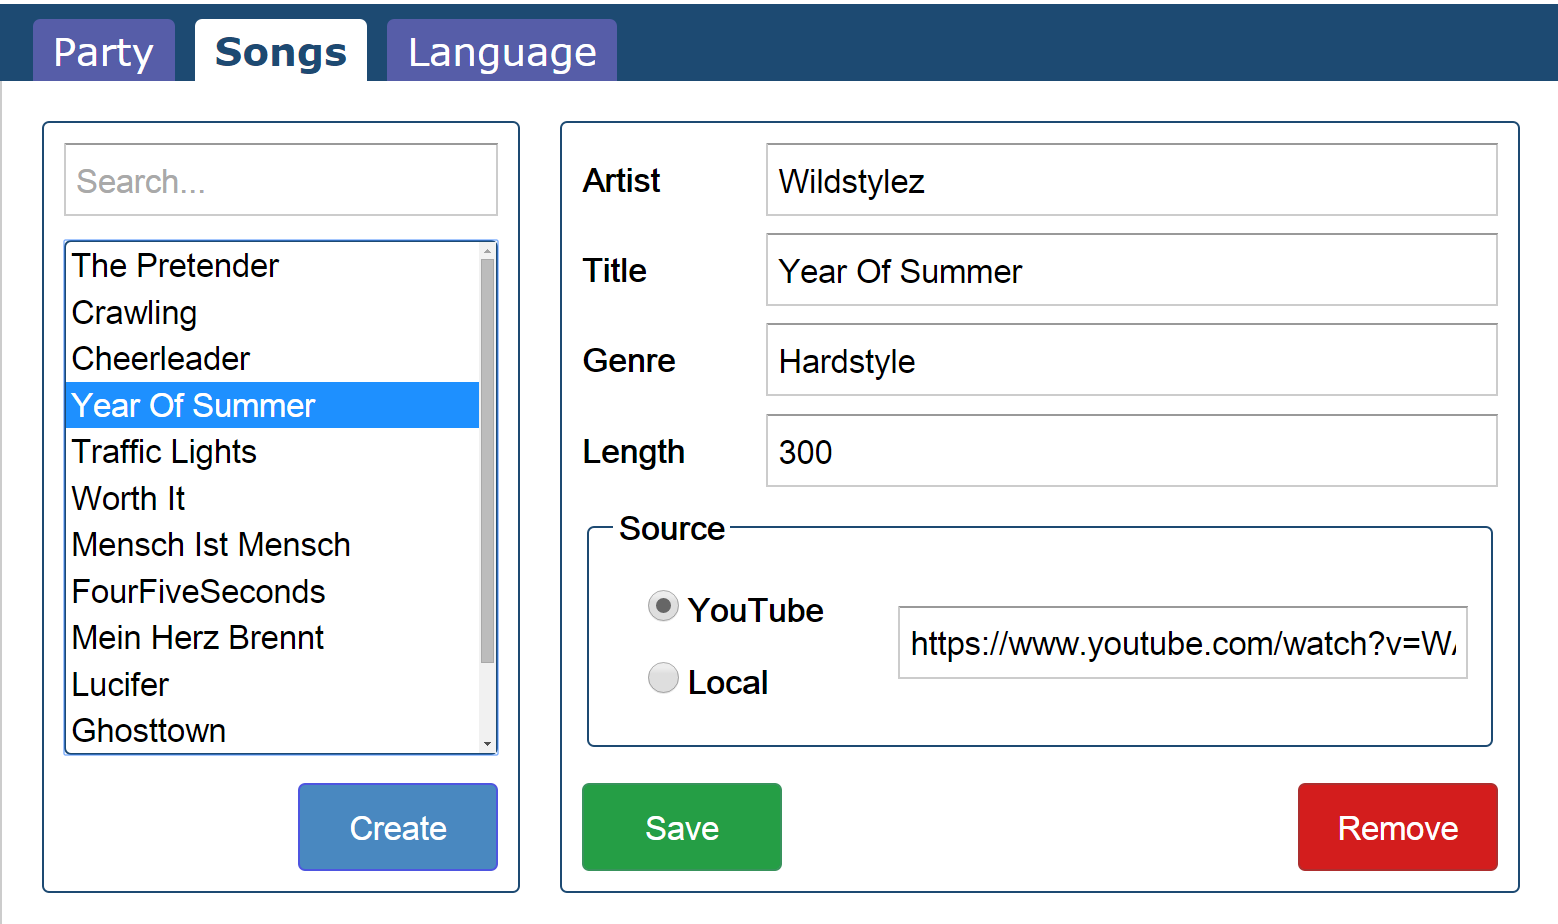
\includegraphics[width=0.9\linewidth]{Bilder/Screenshot-Admin-Songs}
\caption{Screenshot der Oberfläche zur Songverwaltung}
\label{fig:Screenshot-Admin-Songs}
\end{figure}

Die Abbildung \ref{fig:Screenshot-Admin-Songs} zeigt die Verwaltungsoberfläche der Songsammlung aus der Admin-Applikation. Im Vergleich zum Entwurf (Abb. \ref{fig:MockSongVerwaltung}) wurden die Position der Buttons aufgrund der Usability geändert.

\begin{figure}[H]
\centering
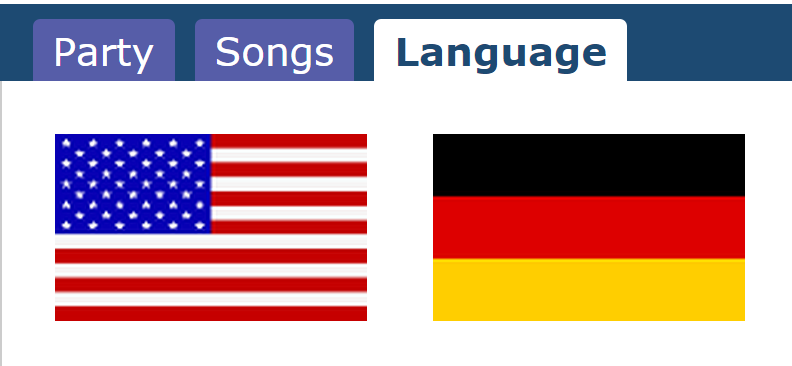
\includegraphics[width=0.5\linewidth]{Bilder/Screenshot-Admin-Language}
\caption{Screenshot der Oberfläche zur Sprachauswahl}
\label{fig:Screenshot-Admin-Language}
\end{figure}

Die Abbildung \ref{fig:Screenshot-Admin-Language} zeigt die Oberfläche für die Sprachauswahl. Aus Gründen der Verständlichkeit wurden die Buttons durch entsprechende Bilder, die die jeweilige Sprache repräsentieren, ersetzt.

\newpage
\subsection{VoteApp}
Die VoteApp orientiert sich im Ergebnis sehr stark an den Entwürfen. Farbakzente verbessern die Benutzbarkeit und heben wichtige Funktionalitäten hervor.

\begin{figure}[H]
\centering
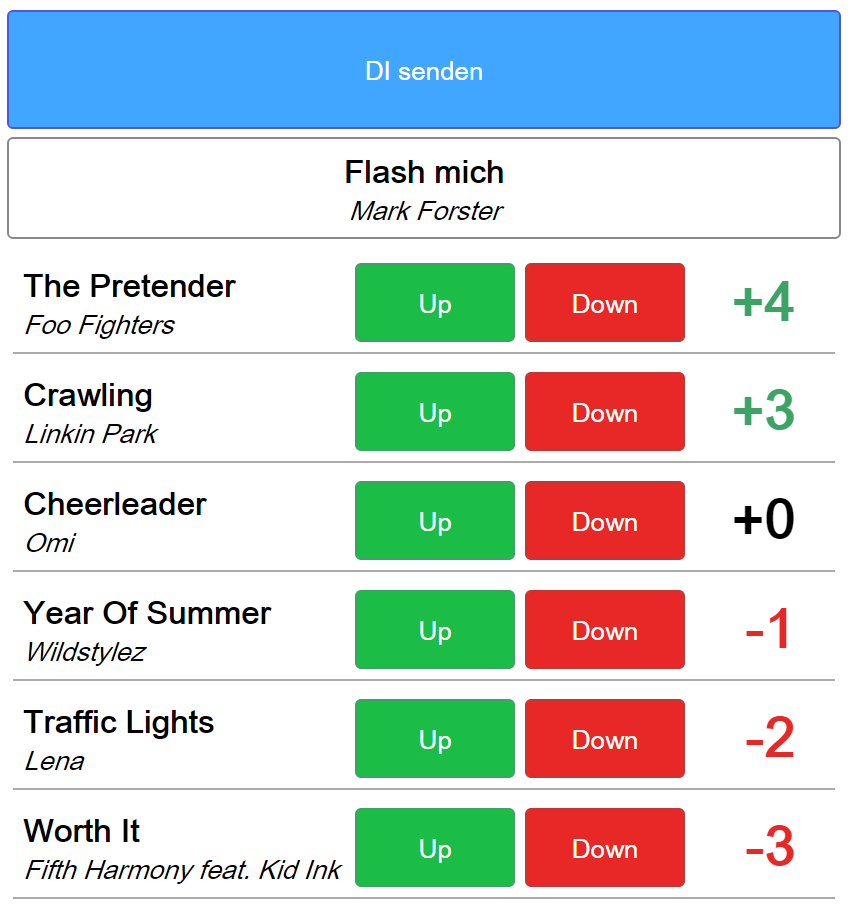
\includegraphics[width=0.5\linewidth]{Bilder/Screenshot-Vote-App}
\caption{Screenshot der VoteApp}
\label{fig:Screenshot-Vote-App}
\end{figure}

Die Abbildung \ref{fig:Screenshot-Vote-App} zeigt die Oberfläche der VoteApp. Diese wurde im Vergleich zum Entwurf (Abb. \ref{fig:MockPartyPeopleClient}) um den Vote-Count erweitert, um dem Anwender eine Rückmeldung auf sein Voting zu geben. Beim Bestätigen der Up- bzw. Down-Buttons wird nun neben dem Vote-Count auch die Position des Songs entsprechend des Votings in der Playlist aktualisiert.

\begin{figure}[H]
\centering
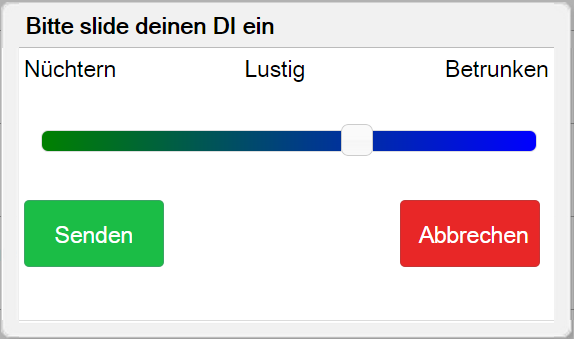
\includegraphics[width=0.45\linewidth]{Bilder/Screenshot-VoteApp-DI-Slider}
\caption{Screenshot des Dialogs zur Eingabe des Drunken-Index}
\label{fig:Screenshot-Vote-App_Slider}
\end{figure}

Die Abbildung \ref{fig:Screenshot-Vote-App_Slider} zeigt den Dialog zur die Eingabe des Drunken-Index der VoteApp. Änderungen im Vergleich zum Entwurf (Abb. \ref{fig:MockDiSlider}) hat es keine gegeben.